% \iffalse
\let\negmedspace\undefined
\let\negthickspace\undefined
\documentclass[journal,12pt,twocolumn]{IEEEtran}
\usepackage{cite}
\usepackage{amsmath,amssymb,amsfonts,amsthm}
\usepackage{algorithmic}
\usepackage{graphicx}
\usepackage{textcomp}
\usepackage{xcolor}
\usepackage{txfonts}
\usepackage{listings}
\usepackage{enumitem}
\usepackage{mathtools}
\usepackage{gensymb}
\usepackage{comment}
\usepackage[breaklinks=true]{hyperref}
\usepackage{tkz-euclide} 
\usepackage{listings}
\usepackage{gvv}                                        
\def\inputGnumericTable{}                                 
\usepackage[latin1]{inputenc}                                
\usepackage{color}                                            
\usepackage{array}                                            
\usepackage{longtable}                                       
\usepackage{calc}                                             
\usepackage{multirow}                                         
\usepackage{hhline}                                           
\usepackage{ifthen}                                           
\usepackage{lscape}
\usepackage{placeins}
\usepackage{xparse}


\newtheorem{theorem}{Theorem}[section]
\newtheorem{problem}{Problem}
\newtheorem{proposition}{Proposition}[section]
\newtheorem{lemma}{Lemma}[section]
\newtheorem{corollary}[theorem]{Corollary}
\newtheorem{example}{Example}[section]
\newtheorem{definition}[problem]{Definition}
\newcommand{\BEQA}{\begin{eqnarray}}
\newcommand{\EEQA}{\end{eqnarray}}
\newcommand{\define}{\stackrel{\triangle}{=}}
\theoremstyle{remark}
\newtheorem{rem}{Remark}

\graphicspath{ {./figs/} } 

\begin{document}

\bibliographystyle{IEEEtran}
\vspace{3cm}

\Large\title{GATE 2022 EE 39}
\large\author{EE23BTECH11032 - Kaustubh Parag Khachane $^{*}$% <-this % stops a space
}
\maketitle
\newpage
\bigskip

\renewcommand{\thefigure}{\theenumi}
\renewcommand{\thetable}{\theenumi}
\large\textbf{Question GATE 22 EE 39} :\\
The damping ratio and undamped natural frequency of a closed loop system as
shown in the figure, are denoted as $\zeta$ and $\omega_n$, respectively. The values of $\zeta$ and $\omega_n$
are 
\begin{figure}[!ht]
\centering
\begin{center}
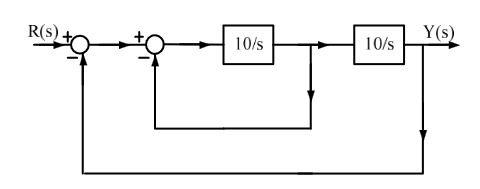
\includegraphics[width=\columnwidth]{question}
\end{center}
%\caption{Diagram for GATE ME Question 30}
\end{figure}
\begin{enumerate}
    \item $\zeta = 0.5$ and $\omega_n = 10$ rad/s
    \item $\zeta = 0.1$ and $\omega_n = 10$ rad/s
    \item $\zeta = 0.707$ and $\omega_n = 10$ rad/s
    \item $\zeta = 0.707$ and $\omega_n = 100$ rad/s
\end{enumerate}
\hfill(GATE EE 2022)\\
\solution\\
\begin{table}[!ht] 
\centering
\setlength{\extrarowheight}{8pt}
\begin{tabular}{|l|l|l|}
    \hline
    \textbf{Parameter} & \textbf{Description} & \textbf{Value} \\
    \hline
     m & Mass of object & 10 Kg \\\hline
     $\mu$ & Frictional coefficient \brak{static} & 0.25\\\hline
     x\brak{t} & Displacement of block &  \\\hline
     $x\brak{0}$ & Initial displacement & 0 \brak{assumed} \\\hline
     g & Gravitational acceleration & 10 $m/s^2$ \\\hline
     $F_s$ & Spring force &  \\\hline
     f & frictional force &  $\mu$ N \\\hline
     N & Normal Force & mg $cos\brak{\theta}$ \\\hline
    \end{tabular}
  \vspace{4mm}
 \caption{Parameter Table}
 \label{tab:table0_xe80}
\end{table}

We will use Mason's Gain Formula to calculate the transfer function of this system. First converting the given diagram to a signal flow graph :
\begin{figure}[!ht]
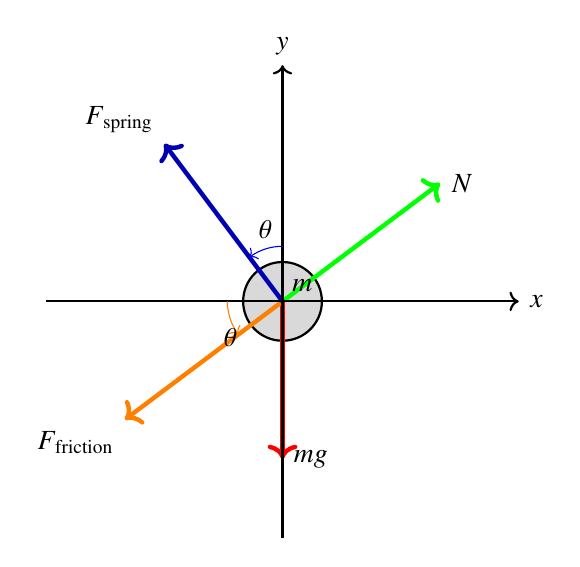
\begin{tikzpicture}
    \centering
    \draw[thick, fill=gray!30] (0,0) circle (0.5cm);
    
    \draw[->, ultra thick, green] (0,0) -- (2,1.5) node[right, black]{$N$};
    \draw[->, ultra thick, red] (0,0) -- (0,-2) node[right, black]{$mg$};
    \draw[->, ultra thick, orange] (0,0) -- (-2,-1.5) node[below left, black]{$F_{\text{friction}}$};
    \draw[->, ultra thick, blue!70!black] (0,0) -- (-1.5,2) node[above left, black]{$F_{\text{spring}}$};    
    
    \node at (0,0) [above right]{$m$};
    
    \draw[->, thick] (-3,0) -- (3,0) node[right]{$x$};
    \draw[->, thick] (0,-3) -- (0,3) node[above]{$y$};
    
    %approximated the angle to 37 degrees theta = 37 deg
    \draw[->, blue] (0,0) ++(90:0.7cm) arc (90:127:0.7cm) node[midway, above, black] {$\theta$};
    \draw[->, orange] (0,0) ++(180:0.7cm) arc (180:217:0.7cm) node[midway, below, black] {$\theta$};
\end{tikzpicture}
\caption{Maximum spring force FBD}
    \label{fig:fig1_xe80}
\end{figure}

Mason's Gain Formula is given by :
\begin{align}
    H\brak{s} = \sum_{i=1}^{N}\brak{\frac{P_i \Delta_i}{\Delta}} \label{eq:eq1_ee39}
\end{align}
\begin{table}[!ht] 
\centering
\setlength{\extrarowheight}{8pt}
\begin{tabular}{|l|l|}
    \hline
    \textbf{Parameter} & \textbf{Description}\\
    \hline
     N & Number of forward paths \\\hline
     L & Number of loops\\\hline
     $P_k$ & Forward path gain of $k^{th}$ path\\\hline
     $\Delta_k$ & Associated path factor \\\hline
     $\Delta$ & Determinant of the graph \\\hline
  \end{tabular}
  \vspace{4mm}
 \caption{Parameter Table - Mason's Gain Law}
 \label{tab:table1_ee_22_39}
\end{table}

\begin{table}[!ht] 
\centering
\setlength{\extrarowheight}{8pt}
\begin{tabular}{|l|l|}
    \hline
    \textbf{Parameter} & \textbf{Formula}\\
    \hline
     $\Delta$ & 1 + $\sum_{k=1}^{L}\brak{\brak{-1}^k\text{Product of gain of groups of k isolated loops}}$ \\\hline
     $\Delta_k$ & $\Delta$ part of graph that is not touching $k^{th}$ forward path \\\hline
  \end{tabular}
  \vspace{4mm}
 \caption{Formula Table - Mason's Gain Law}
 \label{tab:table2_ee_22_39}
\end{table}

This signal flow graph has only one forward path whose gain is given by :
\begin{align}
    P_1 &= \frac{10}{s} \frac{10}{s}\\
    &= \frac{100}{s^2}
\end{align}
The loop gain for loop between Node-2 and Node-3 is :
\begin{align}
    L_1 &= \frac{10}{s}\brak{-1}\\
    &= -\frac{10}{s}
\end{align}
The loop gain for loop between Node-1 and Node-4 is :
\begin{align}
    L_1 &= \frac{10}{s}\frac{10}{s}\brak{-1}\\
    &= -\frac{100}{s^2}
\end{align}
Using \tabref{tab:table2_ee_22_39}, $\Delta$ is :
\begin{align}
    \Delta &= 1 - \brak{-\frac{10}{s} - \frac{100}{s^2}}\\
    &= 1 + \frac{10}{s} + \frac{100}{s^2}
\end{align}
There are no two isolated loops available. Hence all further terms will b zero.\\
As both the loops are in contact with the only forward path,
\begin{align}
    \Delta_1 = 1
\end{align}
Using equation \eqref{eq:eq1_ee39} :
\begin{align}
    H\brak{s} &= \frac{\frac{100}{s^2}}{1 + \frac{10}{s} + \frac{100}{s^2}} \\
    &= \frac{100}{s^2 + 10s + 100}\label{eq:eq2_ee39}
\end{align}
Referring to \tabref{tab:table0_ee_22_39}, the general equation of the damping system is second order and can be written as :
\begin{align}
    m\ddot{y}(t) + c\dot{y}(t) + ky(t) = x(t)
\end{align}
Take the Laplace transform and solve for $\frac{Y\brak{s}}{X\brak{s}}$ :
\begin{align}
    \frac{Y\brak{s}}{X\brak{s}} &= \frac{\omega_n^2}{s^2 + 2\zeta\omega_n s + \omega_n^2}\\
\implies H\brak{s} &= \frac{\omega_n^2}{s^2 + 2\zeta\omega_n s + \omega_n^2} \label{eq:eq3_ee39}
\end{align}
Comparing equations \eqref{eq:eq2_ee39} and \eqref{eq:eq3_ee39} ,
\begin{align}
    \omega_n ^2 &= 100\\
    \implies \omega_n &= 10 \text{ rad/s} \label{eq:eq4_ee39}\\
    2\zeta \omega_n &= 10\\
    \implies \zeta &= 0.5
\end{align}
\begin{figure}[!ht]
\centering
\begin{center}
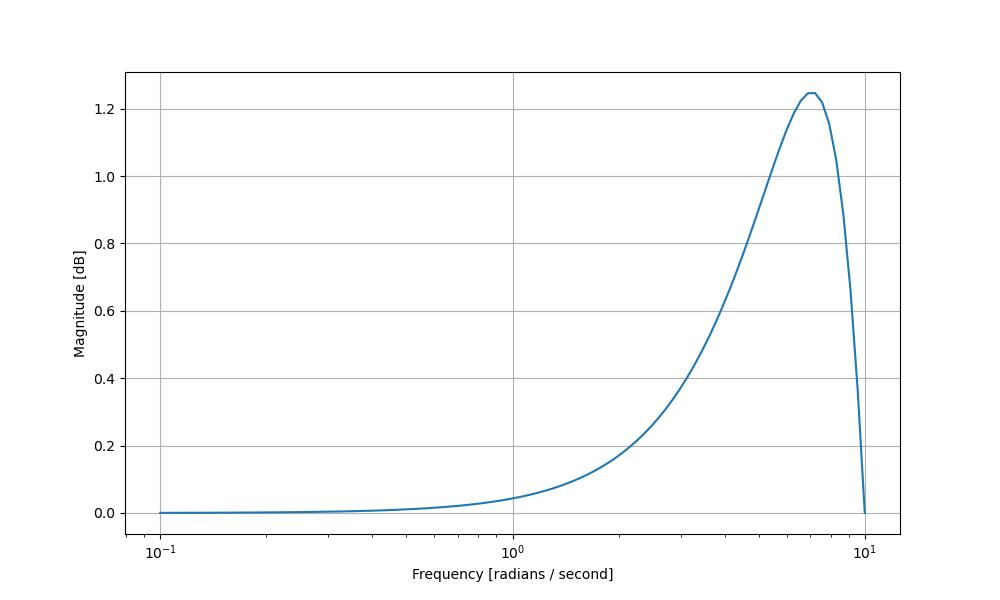
\includegraphics[width=\columnwidth]{Figure_1}
\end{center}
\caption{Magnitude plot}
\end{figure}
\begin{figure}[!ht]
\centering
\begin{center}
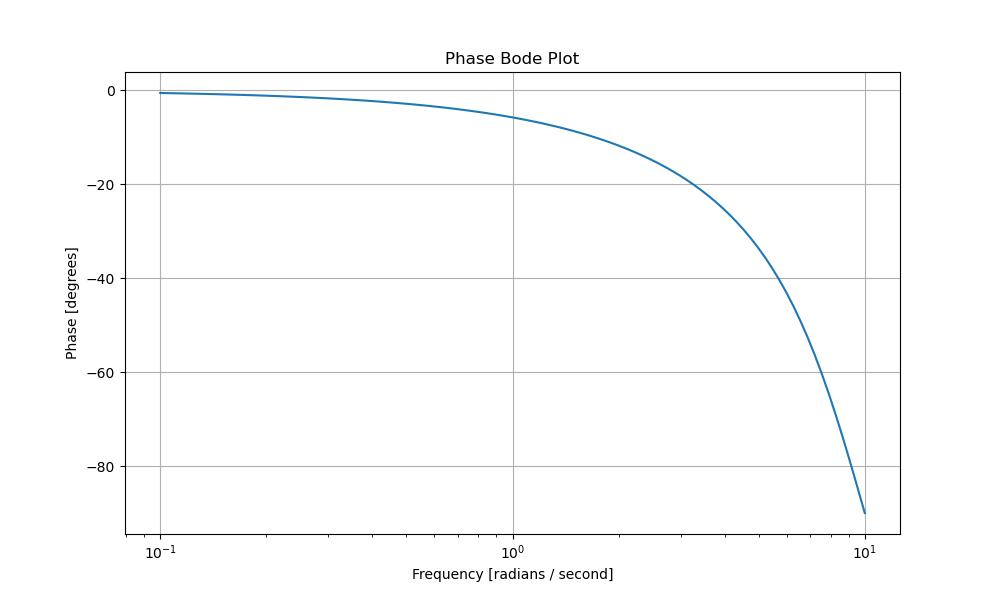
\includegraphics[width=\columnwidth]{Figure_2}
\end{center}
\caption{Phase plot}
\end{figure}
\end{document}
